\documentclass[10pt]{report}
\usepackage{epsf}
\usepackage{amsmath}
\usepackage{amssymb}
\usepackage{float}
\usepackage{palatino}
\usepackage[pdftex]{graphics}
\usepackage{fancyhdr}
\usepackage[pdftex]{graphicx}
\usepackage{hyperref}
\parindent 0in
\parskip 1ex
\oddsidemargin  0in
\evensidemargin 0in
\textheight 8.5in
\textwidth 6.5in
\topmargin -0.25in

\pagestyle{fancy}
\fancyhf{}
\fancyhead[L]{\bf BME354L - Palmeri - Spring 2013}
\fancyhead[R]{{\bf Arduino Project}}
%\fancyfoot[L]{LICENSE: CC BC-NC-SA 3.0 ({\tt http://creativecommons.org/licenses/by-nc-sa/3.0/})}
\fancyfoot[C]{\thepage}

\title{ADC For Embedded Systems}
\author{Will Scheideler}
\begin{document}

\section*{Analog-to-Digital Conversion in Embedded Systems}

\par
	ADC’s are critical components of most embedded systems. ADC’s interface between the continuous electrical signals that are produced by transducers and discrete time signals that a CPU / microcontroller can process in the digital domain. The basic signal processing scheme for embedded systems is this: 

\begin{figure}[H]
\centering
   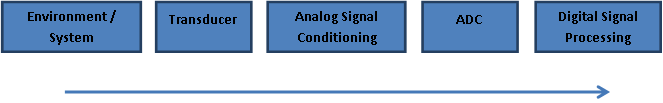
\includegraphics[width=0.7\textwidth]{ADC_1.png}
    \caption{General Scheme for Embedded Systems Signal Processing}
\end{figure}

\par
ADC’s can be found as discrete components or, more commonly, integrated in a microcontroller. Microcontrollers commonly have an on-board ADC of 8-12 bit precision (good enough for most applications). ADC’s are also packaged as discrete components which can be used for specific applications that may have different bit depth and bandwidth needs. For BME 354 and your subsequent design courses, you will be using the ADC capabilities of microcontrollers. It is useful to review the key parameters that describe an ADC configuration:

\begin{description}
  \item[Resolution] \hfill \\
  This is the number of bits in the output code of the ADC. This does not strictly determine the performance of the ADC, except that all performance parameters are measured against this theoretical MAX resolution. For an n-bit ADC, n bits is the maximum resolution you can expect. In practice, the resolution of ADC’s is limited to n-1, n-2, or worse, depending on the noise rejection characteristics of the ADC, etc.

  \item[Acquisition Time] \hfill \\
This is the time required to acquire one sample of the analog input voltage. This parameter sets an upper bound on the bandwidth of signals that may be acquired with an ADC. The acquisition time may be fixed or variable, depending on the ADC architecture and application specific demands.

  \item[Analog Source Impedance] \hfill \\
  The network driving the ADC input has a finite output impedance. This puts a lower limit on the acquisition time (acquisition typically begins with the charging of a sample / hold capacitor).
\end{description}


\subsection*{Arduino UNO ADC}
	The Arduino UNO platform uses an ATMEGA microcontroller, the ATMEGA328, which has a 10-bit ADC. If we refer to the datasheet for the ATMEGA328, we can observe the other characteristics of the ADC. ATMEL lists a maximum of 15kSPS (15k samples per second) when the 10-bit ADC is operated at maximum resolution. The other important feature of the ATMEGA328 ADC module is a ‘flexible multiplexer’ which allows the ADC to reference values from different sources, including an externally applied voltage on Pin AREF, VDD, or a fixed internal reference voltage (~1.1V). This can allow greater precision than simply having a GND - VDD input range. The acquisition time of the ATMEGA328 ADC is a function of the input voltage. The Datasheet says that the ADC takes from 13 µs to 260 µs for conversion. This dependence is a result of the use of a Successive Approximation ADC, which generates an output based on a series of comparisons to dynamically generated voltages. The time that it takes this binary search algorithm to find the input voltage scales logarithmically with the number of bits and has some variation with the value of the input voltage.

%\begin{figure}[H]
%\centering
  % 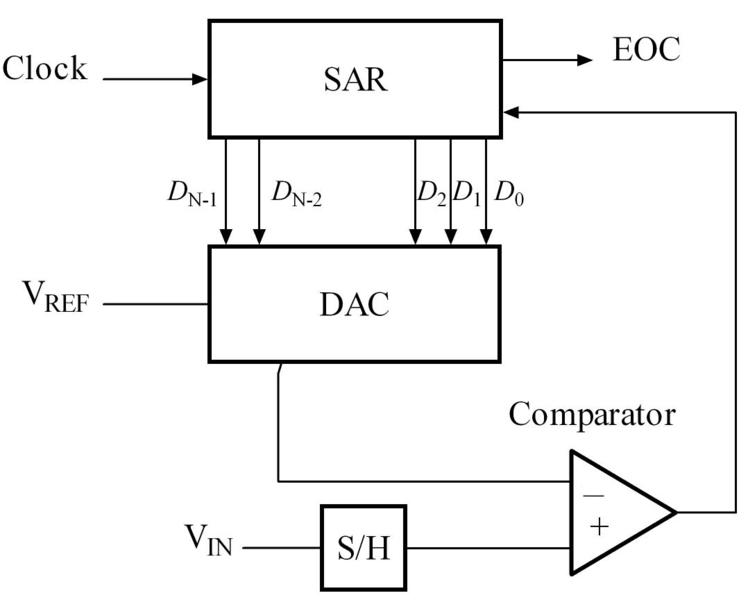
\includegraphics[width=0.9\textwidth]{ADC_2}
    %\caption{Successive Approximation High Level Block Diagram}
%\end{figure}

\end{document}